\documentclass[a4paper]{article}
\usepackage[left=1cm, right=1cm, top=1cm, bottom=1cm]{geometry}
% put the command
%
% \input{odl_preamble.tex}
%
% at the top of your latex file (just after the \documentclass) to include this
% in your document.  Feel free to add to this file, but please consider adding
% commands and packages that are specific to your work outside of this file:
% let's reserve this file for stuff that most of us would need.

% The amssymb package provides various useful mathematical symbols
\usepackage{amsmath}
\usepackage{amsfonts}
\usepackage{amssymb}
\usepackage{amsthm}
\usepackage{graphicx} % for includegraphics
\usepackage{xspace} % needed for \eg, \ie, \etc
\usepackage{bm} % for bold math
%\usepackage{threeparttable} % for tables with footnotes
\usepackage{subcaption}
\usepackage{caption}
\usepackage{graphicx}
\usepackage{fullpage}
\usepackage{textcomp}
\usepackage{listings}
\usepackage{xcolor}
\usepackage{float}
\usepackage{stmaryrd}
\usepackage[toc,page]{appendix}

\usepackage[ruled,lined,linesnumbered]{algorithm2e}

% hyperref must be last
\usepackage{hyperref}
\hypersetup{
  colorlinks=true,
  linkcolor=red,
  citecolor=green,
  urlcolor=blue
}
  
% We often use mathcal for functions
\newcommand{\fnc}[1]{\ensuremath{\mathcal{#1}}}
\newcommand{\vecfnc}[1]{\ensuremath{\boldsymbol{\mathcal{#1}}}} % vector function

% matrices are often math sans serif type
\newcommand{\mat}[1]{\ensuremath{\mathsf{#1}}}

\newcommand{\Pm}[0]{\psi_h^{(n-1)}}
\newcommand{\Pn}[0]{\psi_h^{(n)}}
\newcommand{\Pnn}[0]{\psi_h^{(n+1)}}
\newcommand{\Qn}[0]{q_h^{(n)}}
\newcommand{\Qnn}[0]{q_h^{(n+1)}}

\newcommand{\Sn}[0]{s_h^{(n)}}
\newcommand{\Snn}[0]{s_h^{(n+1)}}
\newcommand{\Lht}[0]{L_{h,\Delta t}}

% SBP operator matrices
\newcommand{\M}[0]{\mat{M}}
\newcommand{\Dx}[0]{\mat{D}_{x}}
\newcommand{\Dy}[0]{\mat{D}_{y}}
\newcommand{\Dz}[0]{\mat{D}_{z}}
\newcommand{\Sx}[0]{\mat{S}_{x}}
\newcommand{\Sy}[0]{\mat{S}_{y}}
\newcommand{\Sz}[0]{\mat{S}_{z}}
\newcommand{\Qx}[0]{\mat{Q}_{x}}
\newcommand{\Qy}[0]{\mat{Q}_{y}}
\newcommand{\Qz}[0]{\mat{Q}_{z}}
\newcommand{\Ex}[0]{\mat{E}_{x}}
\newcommand{\Ey}[0]{\mat{E}_{y}}
\newcommand{\Ez}[0]{\mat{E}_{z}}
\newcommand{\Par}[2]{\frac{\partial {#1}}{\partial{#2}}}
% optimization commands
\newcommand{\Lag}[0]{\fnc{L}}
\newcommand{\optmin}{\ensuremath{\text{minimize}}}
\newcommand{\wrt}{\ensuremath{\text{with respect to}}}
\newcommand{\st}[0]{\ensuremath{\text{s.t.}}}
\newcommand{\W}[0]{\mat{W}} % Hessian
\newcommand{\A}[0]{\mat{A}} % Jacobian
\newcommand{\K}[0]{\mat{K}} % KKT matrix
\newcommand{\Hess}[0]{\mat{H}} % upper Hessenberg
\newcommand{\I}[0]{\mat{I}} % identity
\newcommand{\diff}[0]{\mathrm{d}}
% common math operators
\DeclareMathOperator{\spn}{span}
\DeclareMathOperator{\range}{range}
\DeclareMathOperator{\mydiag}{diag}
\newcommand{\argmin}[0]{\ensuremath{\operatornamewithlimits{argmin}}}
\newcommand{\sgn}[0]{\operatorname{sgn}}
\newcommand{\nullsp}[0]{\operatorname{null}}

% environments for definitions, therorems, etc 
\newtheorem{definition}{Definition}
\newtheorem{proposition}{Proposition}
\newtheorem{corollary}{Corollary}
\newtheorem{lemma}{Lemma}
\newtheorem{remark}{Remark}
\newtheorem{assumption}{Assumption}
\newtheorem{thrm}{Theorem}

% command latin phrases and other short-forms
\newcommand{\etal}[0]{{\em et~al.\@}\xspace}
\newcommand{\eg}[0]{{e.g.\@}\xspace}
\newcommand{\ie}[0]{{i.e.\@}\xspace}
\newcommand{\viz}[0]{{viz.\@}\xspace}
\newcommand{\resp}[0]{{resp.\@}\xspace}

\newcommand{\Jump}[1]{\llbracket #1\rrbracket}
\newcommand{\Mean}[1]{\{\{#1\}\}}
% Misc. commands
\newcommand{\ignore}[1]{} % comment out large sections of code


\title{Assignment 1: Adjoint of Elliptic Equation}
\author{ID:4873}
\begin{document}
 \maketitle
 
\begin{abstract}
  
\end{abstract}

\section{Code summary}
\subsection{Development}
For this assignment, the following functionalities have been implemented:
\begin{itemize}
  \item evaluation of the Jacobian matrix of type \textbf{SparseMatrixCSC} using a coloring complex-step approach;
  \item Newton iteration to solve the nonlinear system;
  \item evaluation of the partial derivative of functionals with respect to the area using the complex-step approach;
  \item evaluation of the partial derivative of residual with respect to the area using the complex-step approach;
  \item adjoint solve;
  \item evaluation of total derivative of functionals.
\end{itemize}
\subsection{How to run the code}
For convergence study of functional, run

\hspace{1cm}\texttt{julia convergence\_study.jl},\\ 
and the results are under directory \textit{results/functional}.
For adjoint solution, run
 
\hspace{1cm}\texttt{julia solve\_adjoint.jl}, \\
and results are under directory \textit{results/adjoints}.

\section{Convergence study of functional}
The convergence study of two functionals, $J_{1,h}$ and $J_{2,h}$, is carried out, with $p=1\sim4$. This requires solving the nonlinear system first. Here both explicit and implicit methods are tried. The results are quite the same as long as the convergence tolerance of Runge-Kutta is set to very small, say, $10^{-13}$. 

The results are shown in Figure~\ref{fig:conv_study}. As seen, the error in $J_{1,h}$ sees superconvergence while the error in $J_{2,h}$ does not. Specifically, for $J_{1,h}$ the observed convergence rates with $p=1,2$ are $2p$ while with $p=3,4$ the convergence rates are even higher than $2p$ before the functional error reaches machine zero.
On the contrary, the convergence rates for $J_{2,h}$ are uniformly $p+1$. These results indicate that,
\begin{itemize}
  \item the discretization is probably adjoint consistent;
  \item the adjoint solution of functional $J_{1,h}$ is smooth while that of $J_{2,h}$ is not.
\end{itemize}

\begin{figure}[!htbp]
	\centering
	\begin{subfigure}{0.45\textwidth}
		\centering
		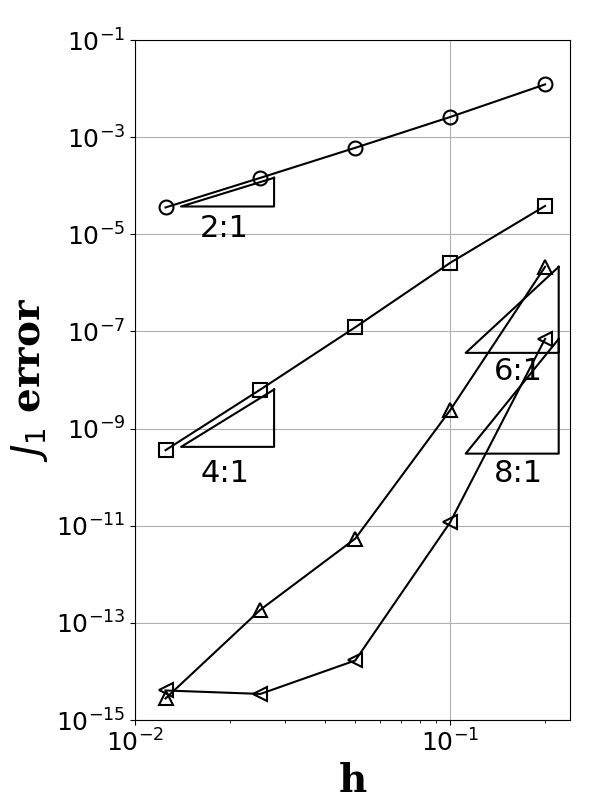
\includegraphics[width=1.0\linewidth]{figures/implicit_J1_error.png}
		\subcaption{$J_{1,h}$ error}
		\label{fig:j1_error}
	\end{subfigure}
	\begin{subfigure}{0.45\textwidth}
		\centering
		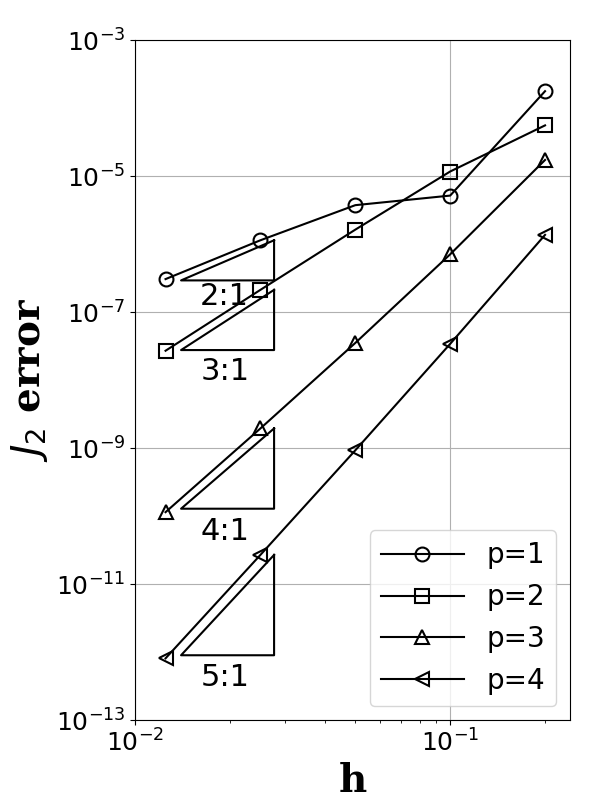
\includegraphics[width=1.0\linewidth]{figures/implicit_J2_error.png}
		\subcaption{$J_{2,h}$ error}
		\label{fig:j2_error}
	\end{subfigure}
	\caption{Functional errors} 
	\label{fig:conv_study}
\end{figure}

\section{Adjoints of $J_{1,h}$ and $J_{2,h}$}
The adjoint solve requires the evaluation of the Jacobian matrix of the nonlinear system. As aforementioned, a coloring complex-step method is implemented. For this specific problem, elements $i, i+3, i+6,\dots$, are grouped together, resulting three colors totally. With number of degrees of freedom per element being $N_{dof,elem}$, the evaluation of Jacobian matrix requires only $3N_{dof,elem}$ residual evaluations. 

With the Jacobian matrix available, a raw Newton iteration is implemented to solve the nonlinear system, as an alternative to the explicit Runge-Kutta. Although no effort is spend to improve the robustness, no convergence problem has been encountered for all the test cases shown in this assignment. Compared to the explicit methods, the implicit method is usually dozens times faster, especially for large cases.

Similar to the evaluation of Jacobian matrix, the derivative of functionals with respect to the solution $q_h$, $\partial J_{i,h}/\partial q_{h}$ is also evaluated using complex-step. Finally, the linear adjoint system is solved using a direct solver.

Although several difference grids are used to ensure the solution is grid independent, only results on \texttt{numelem=100} are displayed here. 

The adjoints of $J_{1,h}$ and $J_{2,h}$ are plotted in Figure~\ref{fig:j1_phi} and \ref{fig:j2_phi}, respectively. Obviously, with \texttt{numelem=100}, all the adjoint solutions coincide with each other, which indicates that the mesh is sufficiently refined. The only exception occurs near $x=1$ in Figure~\ref{fig:j2_phi}.

The adjoints of $J_{1,h}$ are all smooth, while the adjoints of $J_{2,h}$ see severe oscillations near $x=1$. These oscillations destroy the smoothness of the adjoint solution, which is one of the prerequisites to obtain superconvergence in evaluation of functionals. This is why in Figure~\ref{fig:j2_error} the convergence rates of $J_{2,h}$ are $p+1$ rather than $2p$.
\begin{figure}[!htbp]
  \centering
  \begin{subfigure}{0.45\textwidth}
    \centering
    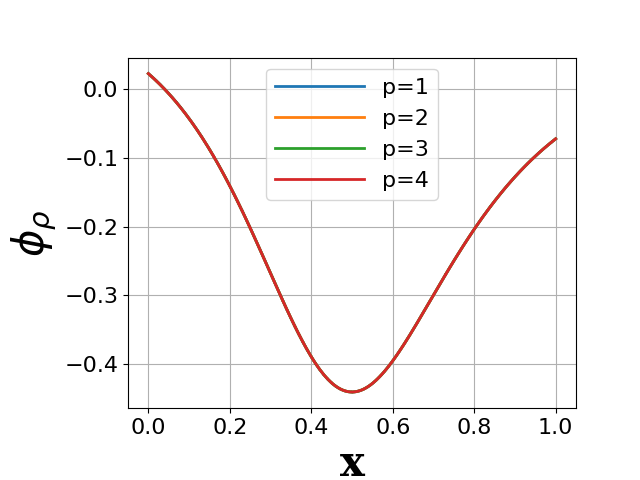
\includegraphics[width=1.0\linewidth]{figures/J1_phi_1.png}
    \subcaption{$\phi_\rho$ of $J_{1,h}$}
    \label{fig:j1_phi1}
  \end{subfigure}
  \begin{subfigure}{0.45\textwidth}
    \centering
    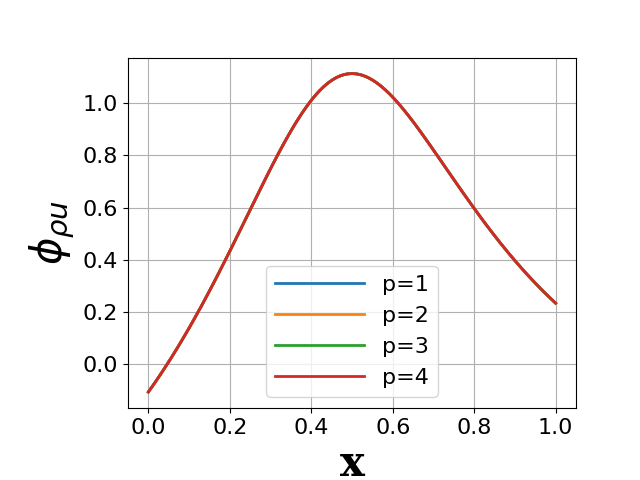
\includegraphics[width=1.0\linewidth]{figures/J1_phi_2.png}
    \subcaption{$\phi_{\rho u}$ of $J_{1,h}$}
    \label{fig:j1_phi2}
  \end{subfigure}
\begin{subfigure}{0.45\textwidth}
  \centering
  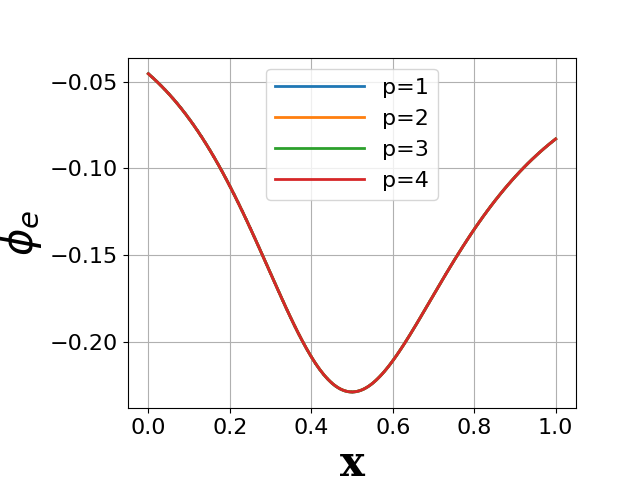
\includegraphics[width=1.0\linewidth]{figures/J1_phi_3.png}
  \subcaption{$\phi_e$ of $J_{1,h}$}
  \label{fig:j1_phi3}
\end{subfigure}
  \caption{Adjoints of $J_{1,h}$} 
  \label{fig:j1_phi}
\end{figure}


\begin{figure}[!htbp]
  \centering
  \begin{subfigure}{0.45\textwidth}
    \centering
    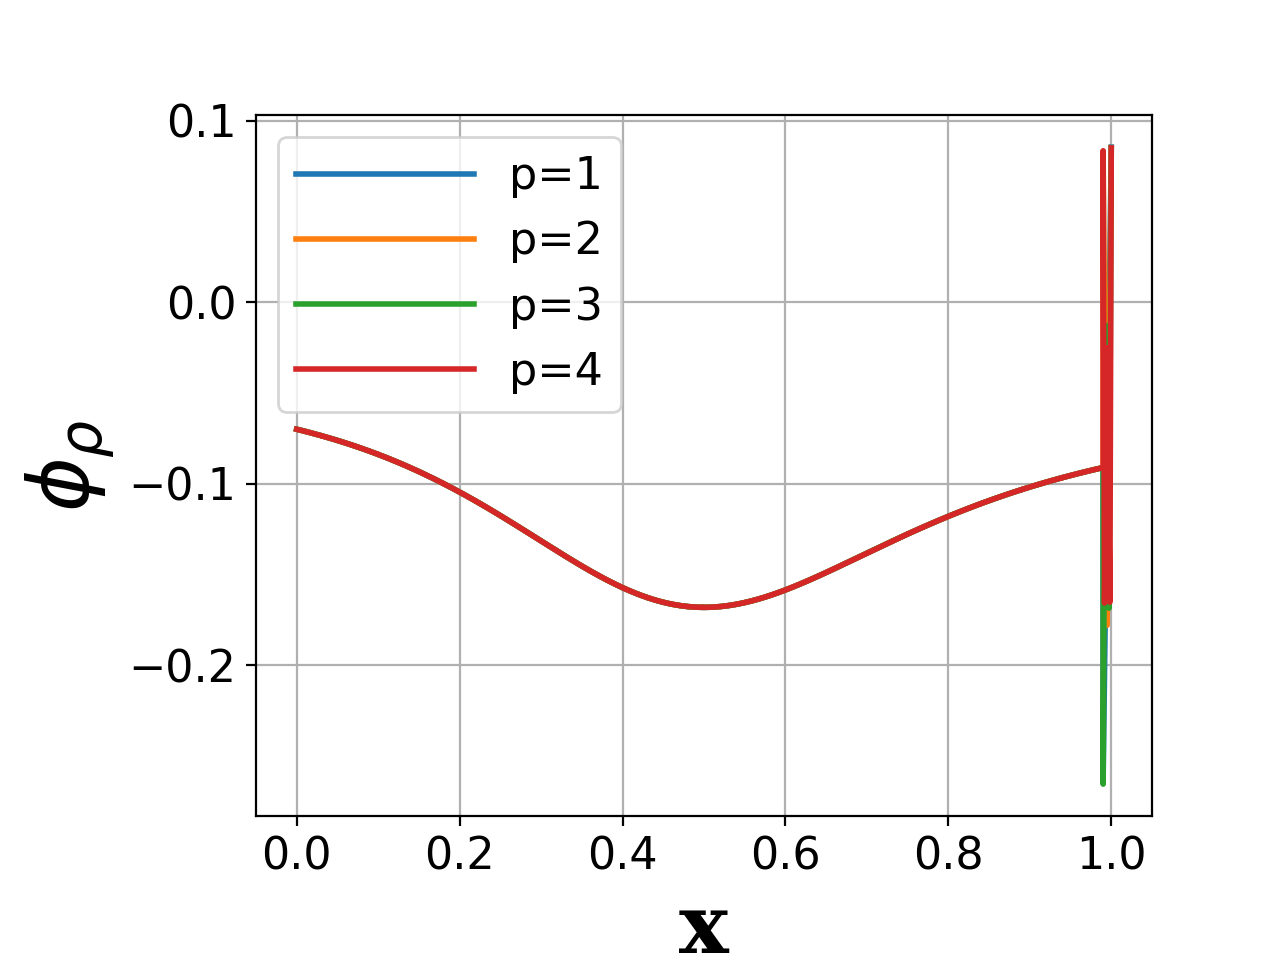
\includegraphics[width=1.0\linewidth]{figures/J2_phi_1.png}
    \subcaption{$\phi_\rho$ of $J_{2,h}$}
    \label{fig:j2_phi1}
  \end{subfigure}
  \begin{subfigure}{0.45\textwidth}
    \centering
    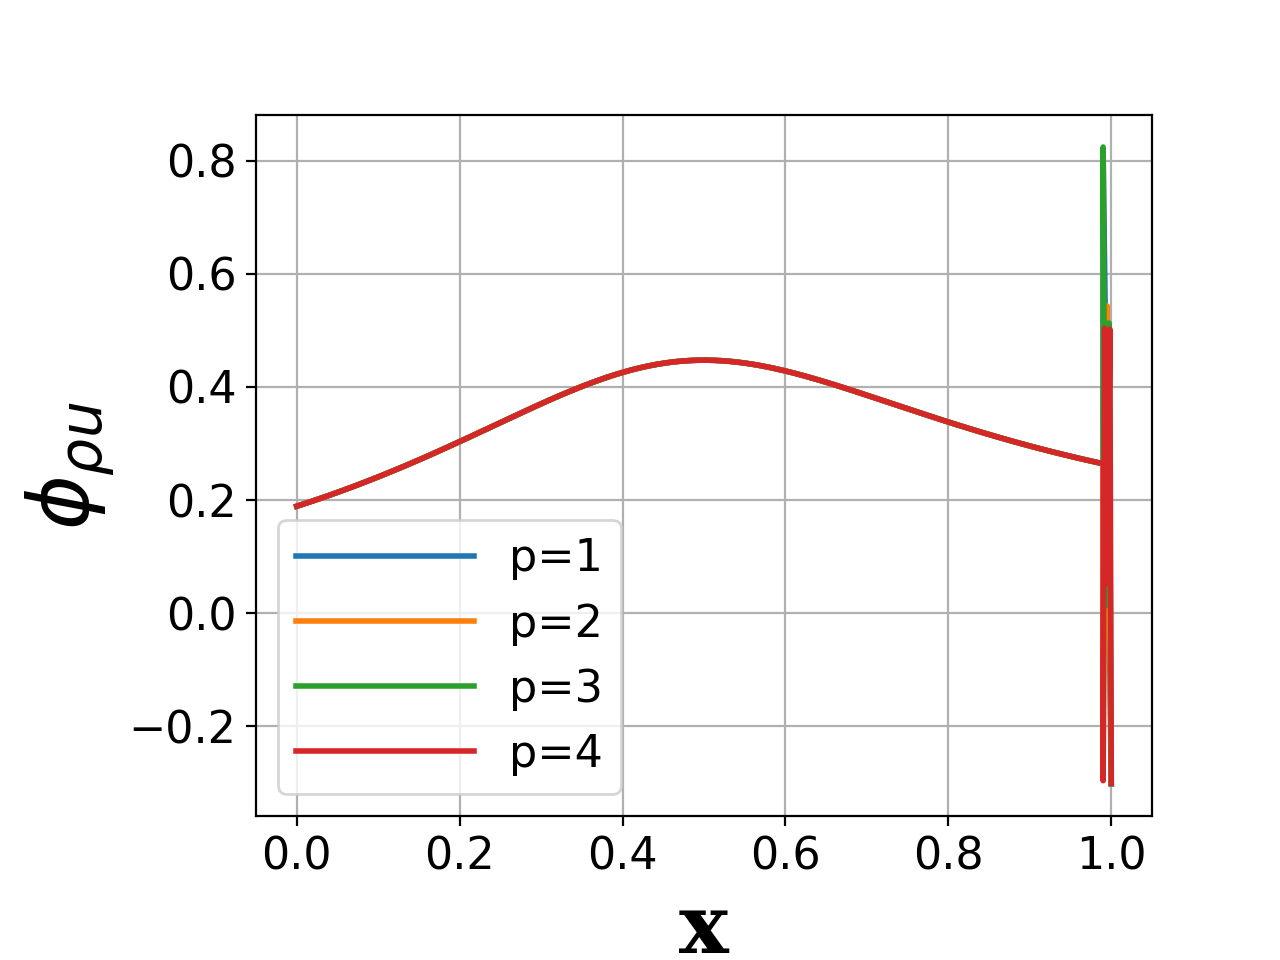
\includegraphics[width=1.0\linewidth]{figures/J2_phi_2.png}
    \subcaption{$\phi_{\rho u}$ of $J_{2,h}$}
    \label{fig:j2_phi2}
  \end{subfigure}
  \begin{subfigure}{0.45\textwidth}
    \centering
    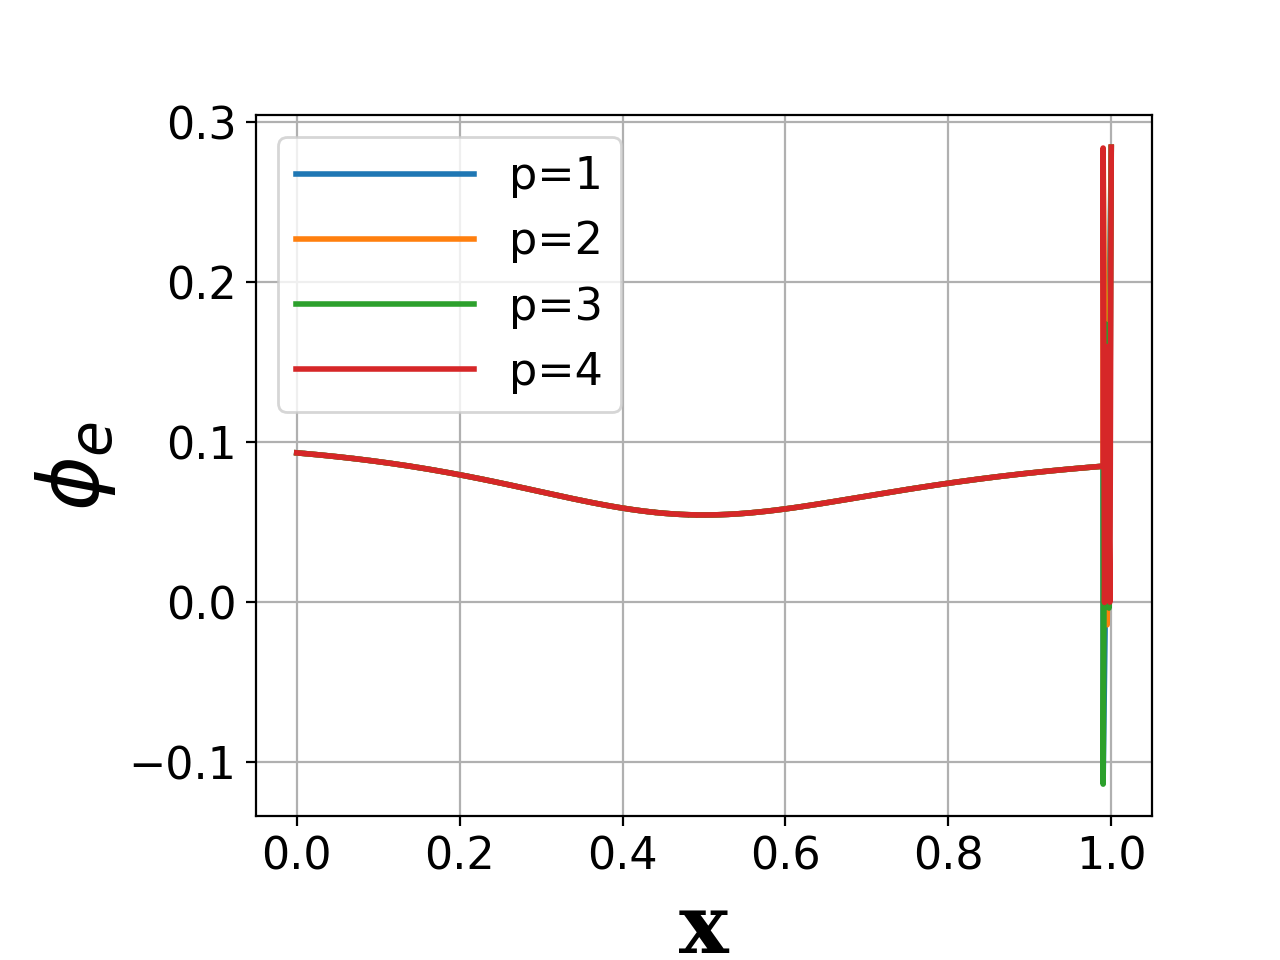
\includegraphics[width=1.0\linewidth]{figures/J2_phi_3.png}
    \subcaption{$\phi_e$ of $J_{2,h}$}
    \label{fig:j2_phi3}
  \end{subfigure}
  \caption{Adjoints of $J_{2,h}$} 
  \label{fig:j2_phi}
\end{figure}

\section{Evaluation of total derivatives of functionals}
Based on the adoint solution, the total derivatives of $J_{1,h}$ and $J_{2,h}$ with respect to the area, $\frac{DJ_{i,h}}{DA}$, are computed. The results are plotted in Figure~\ref{fig:dJ1dA} and \ref{fig:dJ2dA}.
As seen, for both cases, the derivatives are close to zero except inside the first and last elements. For $J_{1,h}$, this can be easy explain as follows:
By integration by parts, 
\begin{equation*}
J_1 = (pA)|^{1}_{0} - \int_{0}^{1}\frac{\partial p}{\partial x}A\diff x
\end{equation*}
Assuming the area is smooth along $x$, $\frac{\partial p}{\partial x}$ is small for subsonic flow, then
\begin{equation*}
\frac{DJ_1}{DA} \approx \begin{cases}
0, 0<x<1 \\
p, x=0,1
\end{cases}
\end{equation*} 
\begin{figure}[!htbp]
  \centering
  \begin{subfigure}{0.45\textwidth}
    \centering
    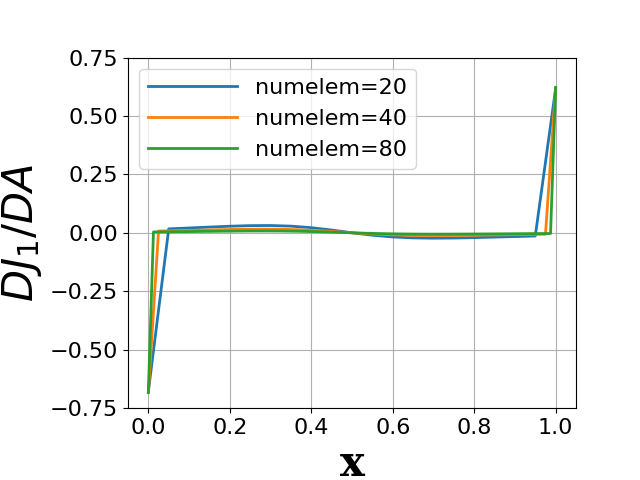
\includegraphics[width=1.0\linewidth]{figures/DJ1DA_p1.png}
    \subcaption{$p=1$}
    \label{fig:Dj1_p1}
  \end{subfigure}
  \begin{subfigure}{0.45\textwidth}
    \centering
    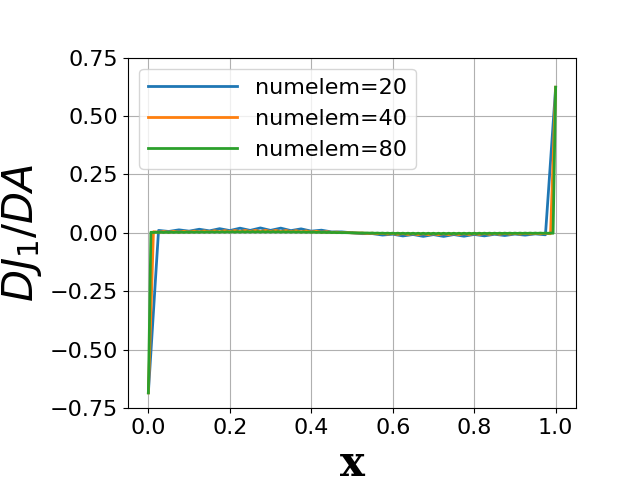
\includegraphics[width=1.0\linewidth]{figures/DJ1DA_p2.png}
    \subcaption{$p=2$}
    \label{fig:Dj1_p2}
  \end{subfigure}
  \begin{subfigure}{0.45\textwidth}
    \centering
    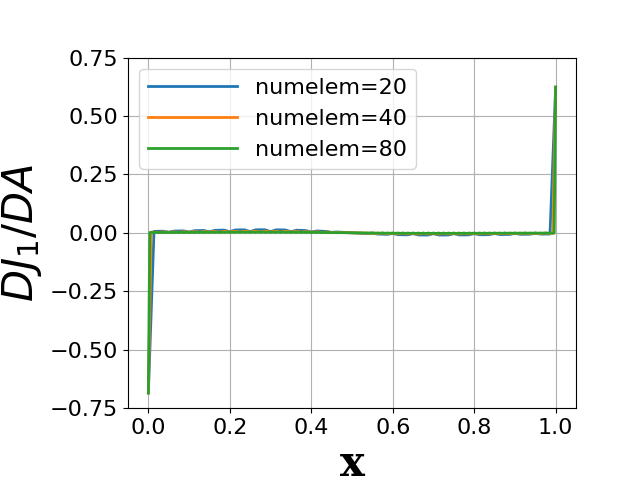
\includegraphics[width=1.0\linewidth]{figures/DJ1DA_p3.png}
    \subcaption{$p=3$}
    \label{fig:Dj1_p3}
  \end{subfigure}
  \begin{subfigure}{0.45\textwidth}
    \centering
    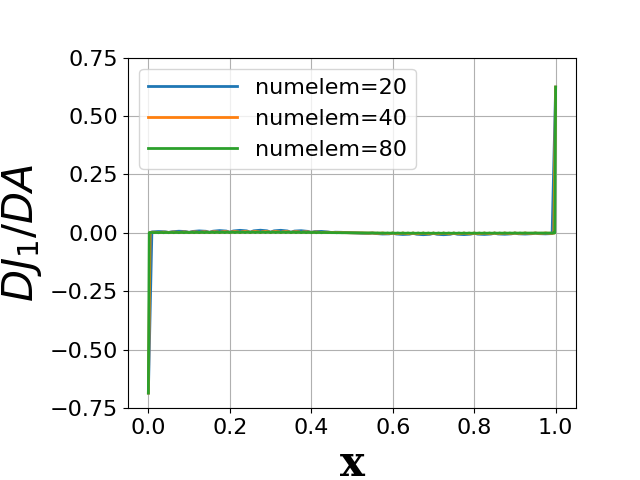
\includegraphics[width=1.0\linewidth]{figures/DJ1DA_p4.png}
    \subcaption{$p=4$}
    \label{fig:Dj1_p4}
  \end{subfigure}
  \caption{Value of $\frac{DJ_1}{DA}$} 
  \label{fig:dJ1dA}
\end{figure}

\begin{figure}[!htbp]
  \centering
  \begin{subfigure}{0.45\textwidth}
    \centering
    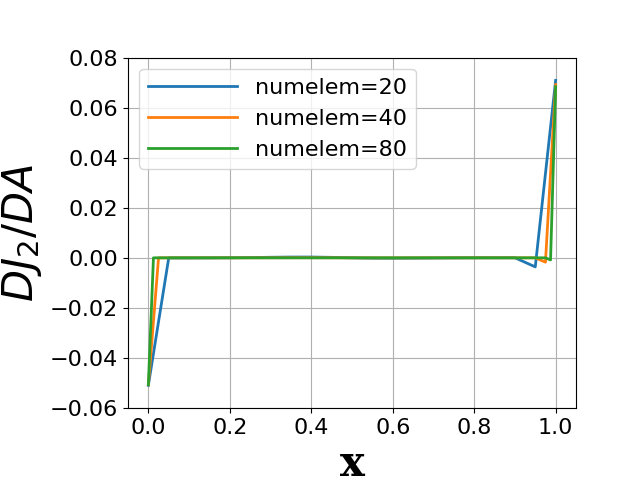
\includegraphics[width=1.0\linewidth]{figures/DJ2DA_p1.png}
    \subcaption{$p=1$}
    \label{fig:Dj2_p1}
  \end{subfigure}
  \begin{subfigure}{0.45\textwidth}
    \centering
    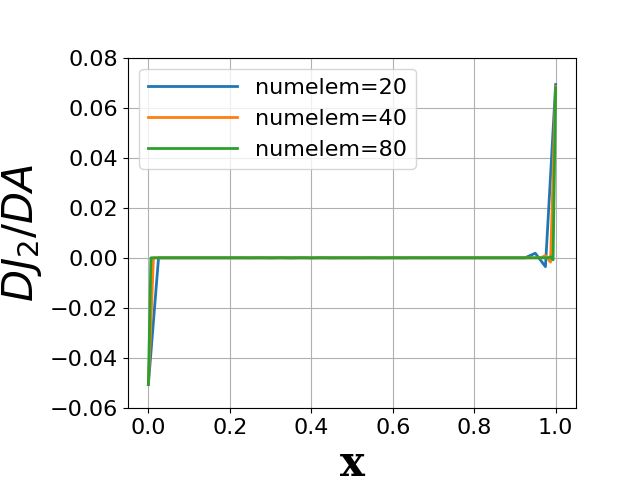
\includegraphics[width=1.0\linewidth]{figures/DJ2DA_p2.png}
    \subcaption{$p=2$}
    \label{fig:Dj2_p2}
  \end{subfigure}
  \begin{subfigure}{0.45\textwidth}
    \centering
    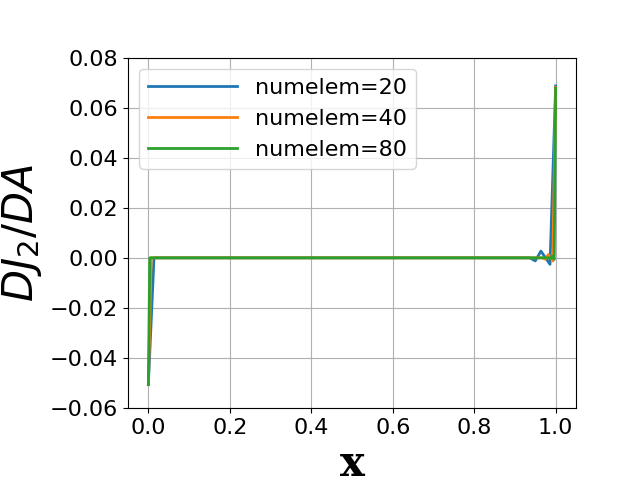
\includegraphics[width=1.0\linewidth]{figures/DJ2DA_p3.png}
    \subcaption{$p=3$}
    \label{fig:Dj2_p3}
  \end{subfigure}
  \begin{subfigure}{0.45\textwidth}
    \centering
    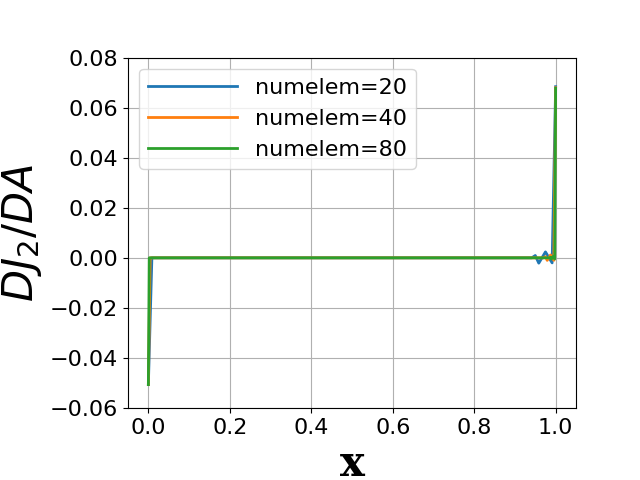
\includegraphics[width=1.0\linewidth]{figures/DJ2DA_p4.png}
    \subcaption{$p=4$}
    \label{fig:Dj2_p4}
  \end{subfigure}
  \caption{Value of $\frac{DJ_2}{DA}$} 
  \label{fig:dJ2dA}
\end{figure}

\bibliographystyle{aiaa}
\bibliography{reference}
\end{document}

